
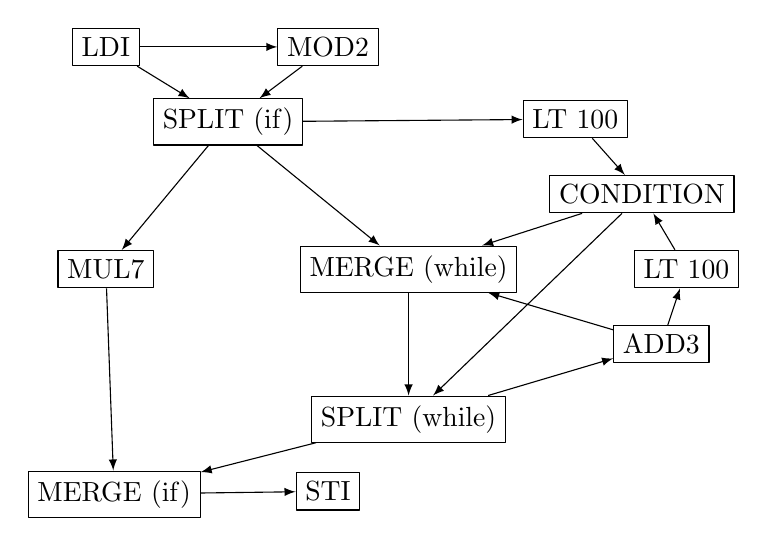
\begin{tikzpicture}[>=latex,line join=bevel,]
%%
\node (lt2) at (249bp,114bp) [draw,rectangle] {LT 100};
  \node (mod2) at (120bp,194bp) [draw,rectangle] {MOD2};
  \node (add3) at (240bp,87bp) [draw,rectangle] {ADD3};
  \node (c) at (233bp,141bp) [draw,rectangle] {CONDITION};
  \node (bm) at (43bp,33bp) [draw,rectangle] {MERGE (if)};
  \node (ldi) at (40bp,194bp) [draw,rectangle] {LDI};
  \node (lm) at (149bp,114bp) [draw,rectangle] {MERGE (while)};
  \node (lt1) at (209bp,168bp) [draw,rectangle] {LT 100};
  \node (sti) at (120bp,34bp) [draw,rectangle] {STI};
  \node (ls) at (149bp,60bp) [draw,rectangle] {SPLIT (while)};
  \node (bs) at (84bp,167bp) [draw,rectangle] {SPLIT (if)};
  \node (mul7) at (40bp,114bp) [draw,rectangle] {MUL7};
  \draw [->,solid] (bm) -- (sti);
  \draw [->,solid] (add3) -- (lm);
  \draw [->,solid] (lt2) -- (c);
  \draw [->,solid] (bs) -- (lm);
  \draw [->,solid] (c) -- (ls);
  \draw [->,solid] (bs) -- (mul7);
  \draw [->,solid] (c) -- (lm);
  \draw [->,solid] (lt1) -- (c);
  \draw [->,solid] (bs) -- (lt1);
  \draw [->,solid] (mod2) -- (bs);
  \draw [->,solid] (ls) -- (bm);
  \draw [->,solid] (add3) -- (lt2);
  \draw [->,solid] (lm) -- (ls);
  \draw [->,solid] (mul7) -- (bm);
  \draw [->,solid] (ldi) -- (bs);
  \draw [->,solid] (ls) -- (add3);
  \draw [->,solid] (ldi) -- (mod2);
%
\end{tikzpicture}

